\documentclass[
  letterpaper,
  DIV=11,
  numbers=noendperiod]{scrartcl}

\usepackage{amsmath,amssymb}
\usepackage{xcolor}
\usepackage{graphicx}
\usepackage{longtable}
\usepackage{booktabs}
\usepackage{array}
\usepackage{bookmark}
\usepackage[round]{natbib}
\usepackage{microtype}
\usepackage{xurl}
\usepackage{siunitx} 

\hypersetup{
  pdftitle={Cultural Matching and the Persistence of Social Ties},
  pdfauthor={Omar Lizardo},
  colorlinks=true,
  linkcolor={blue},
  filecolor={maroon},
  citecolor={blue},
  urlcolor={blue}
}

\title{Cultural Matching and the Persistence of Social Ties}
\author{Omar Lizardo}
\date{\today}

\begin{document}
\maketitle

\begin{abstract}
This paper develops and tests a cultural matching model of social tie persistence using longitudinal ego-network data from the NetSense study. We find that shared cultural tastes serve as a critical mechanism for stabilizing social ties, particularly for weaker relationships, while network opacity—a lack of knowledge regarding an alter's preferences—independently accelerates tie dissolution.
\end{abstract}

\section{Introduction}\label{introduction}

A central puzzle in the sociology of culture and social networks is the co-evolution of social ties and cultural tastes. Traditional sociological models of taste formation posit that an individual's cultural profile is largely a product of their current social network configuration. Tastes are assumed to diffuse through existing homophilous ties, which are themselves structured by socio-demographic similarity---``status homophily'' \citep{lazarsfeld1954, mcpherson2001}. Under this view, ``birds of a feather flock together,'' and due to this mutual flocking, they end up consuming the same cultural goods \citep{mark1998b, mark2003}. Tastes are construed as highly malleable, ``thin'' contents liable to shift whenever the surrounding network ties change. Yet, longitudinal network research reveals that personal networks are constantly in flux, with ties constantly being added, modified, and deleted \citep{burt2000, burt2002, wellman1997}. This empirical fact of network volatility raises a major question: if networks are unstable and tastes are merely thin, network-contingent contents, how do we account for the durable, resilient cultural profiles that individuals maintain over time \citep{bourdieu1984, holt1998}?

In this paper, we develop and test a \textbf{cultural matching model} of tie persistence. We propose that instead of tastes merely adapting to match pre-existing networks, pre-existing cultural dispositions serve as an active ``social glue'' that determines which network ties survive and which dissolve. Under this model, dyadic cultural matching (commonalities in tastes and activities) increases the over-time stability and cognitive salience of social ties, net of usual dyadic determinants such as subjective closeness and tie duration. Using rich longitudinal ego-network data from the NetSense study, we track the persistence of social ties across multiple college-year transitions. To isolate peer dynamics, we restrict our focus to non-kin, on-campus student ties. We unpack this cultural matching mechanism in two ways. First, we establish the baseline protective effect of aggregate cultural matching on tie persistence. Second, we explore the role of ``network opacity''---the degree to which an ego lacks knowledge of their alter's preferences (indicated by ``Don't Know'' responses)---as an independent predictor of tie decay.

\section{Theoretical Framework}\label{theoretical-framework}

\subsection{Tastes and Social Networks: Two Perspectives}\label{tastes-and-social-networks-two-perspectives}

The relationship between cultural tastes and social networks has been conceptualized in two contrasting ways in sociological theory. The \textbf{network transmission perspective}, drawing on constructural imagery \citep{carley1991}, views tastes as malleable, network-contingent contents \citep{erickson1988, erickson1996, mark1998a, mark2003}. Recent work suggests that this malleability is constrained by deeper, latent cultural structures. In this view, social ties constitute the pre-existing ``infrastructure'' or ``pipes'' through which cultural practices diffuse \citep{borgatti2005, erickson1996}. Tastes are learned, adopted, and abandoned based on continuous exchange of cultural information and local bandwagon imitation within an actor's immediate ego network \citep{mark2003}. Because personal networks exhibit substantial over-time volatility---with 30\% to 60\% turnover annually in most personal networks \citep{morgan1997, suitor1997}---the network transmission perspective implies that individual tastes must exhibit corresponding volatility.

In contrast, the \textbf{cultural capital perspective} conceptualizes tastes as highly durable, embodied dispositions reaped from early socialization \citep{bourdieu1984, bourdieu1990, holt1997, holt1998}. Emphasizing the ``interconvertibility'' of different forms of capital \citep{bourdieu1986}, this view sees cultural aptitudes not merely as by-products of ties, but as fundamental resources that help people form and sustain network connections. Here, networks are seen as fleeting structures built and maintained via interactions \citep{dimaggio1987}, and individuals actively use pre-existing tastes to construct novel relationships or shed culturally incompatible ties \citep{vaisey2010}. If tastes are durable and personal networks are volatile, it is highly probable that tastes serve as \emph{drivers} of network connections rather than being exclusively determined by them. This leads to the concept of \textbf{choice homophily} or cultural matching: new social connections are selected, and existing connections are maintained, based on pre-existing cultural compatibility \citep{lazarsfeld1954, werner1979}. In other words, socio-demographic homophily may frequently operate as a \emph{by-product} of active contact selection keyed around cultural alignment, rather than homophily acting as an exogenous structural constraint \citep{carley1991, dimaggio1987}.

\subsection{Cultural Matching and Tie Persistence}\label{cultural-matching-and-tie-persistence}

A major challenge for any newly formed social relationship is what Burt \citep{burt2000}, drawing on Stinchcombe \citep{stinchcombe1965}, refers to as the \textbf{``liability of newness.''} Newly formed dyadic ties are fragile and exhibit a high baseline hazard of decay (``tie decay''), which steeply declines as a relationship matures and ripens into close friendship. What stabilizes a tie and helps it overcome this liability of newness? While classic network models emphasize structural factors (such as network constraint or multiplexity) and dyadic factors (such as subjective closeness), we propose that \textbf{cultural matching} serves as a vital stabilizing mechanism. Shared tastes and cultural practices provide a common cognitive and behavioral baseline that facilitates smooth, low-cost social interaction \citep{collins2004, dimaggio1987}.

When ego and alter share cultural dispositions, they can engage in shared activities and coordinate behavior with minimal friction. Over time, this cultural alignment increases the cognitive salience of the alter, rendering the tie resistant to decay and facilitating its retention in the ego's active network \citep{burt2000}. Therefore, we expect that commonalities in cultural tastes and leisure practices will significantly reduce the hazard of tie decay, net of subjective closeness and structural controls (\textbf{The Baseline Matching Hypothesis}).

\subsection{Network Opacity}\label{network-opacity}

Finally, we introduce the concept of \textbf{network opacity}. If shared cultural knowledge stabilizes ties, then a lack of mutual cultural knowledge---network opacity---is a diagnostic signal of relationship precarity. When an ego reports ``Don't Know'' regarding an alter's preferences across multiple cultural domains, this indicates a lack of conversational intimacy and shared experiences, which should independently predict a higher hazard of tie dissolution \citep{burt2002, wellman1997}. We test both the main effect of network opacity on tie decay and whether opacity moderates the protective effect of known cultural matches.

\section{Data and Methods}\label{data-and-methods}

Data for this analysis comes from the NetSense study, a longitudinal survey of college students conducted at the University of Notre Dame between 2011 and 2015. The study collected extensive panel data on students' social networks, demographic backgrounds, and cultural preferences. A comprehensive codebook, data dictionary, and repository for the NetSense project are available at \url{https://olizardo.github.io/NetSense-Codebook/}.

We collected information on the cultural habits of ego-alter pairs using both a series of closed-form domain questions and open-ended activity nominations. For the closed-form items, egos were asked to rate both their own and their alters' level of interest across six broad cultural and leisure domains: music, movies, books, sports, games, and outdoor activities. For the open-ended items, respondents freely nominated up to five leisure activities they enjoyed, and then indicated whether their alter also engaged in each nominated activity.

\subsection{Study Waves}\label{study-waves}

The NetSense study is a longitudinal survey of college students collected over multiple waves. For this analysis of tie persistence, we pool data across adjacent waves to construct a person-period dataset. To isolate peer dynamics, we restrict our sample to non-kin, on-campus ties (i.e., alters who are also students at Notre Dame). Specifically, we focus on transitions between: 
\begin{itemize}
    \item \textbf{Wave 1 to Wave 2}: Capturing tie dynamics over the first year of college.
    \item \textbf{Wave 2 to Wave 5}: Spanning the middle years of the college experience (approximately a 3-year gap).
    \item \textbf{Wave 5 to Wave 6}: Capturing the transition through the final year and toward graduation.
\end{itemize}

\subsection{Measures}\label{measures}

\subsubsection{Dependent Variable}
\emph{Tie Persistence}: A binary indicator taking a value of 1 if a social tie reported by an ego in a baseline wave (e.g., Wave 1) is still present in the subsequent wave (e.g., Wave 2), and 0 if the tie has dissolved (i.e., the alter is no longer listed in the ego's network).

\subsubsection{Independent Variables} 
\begin{itemize}
    \item \emph{Closed-Form Cultural Matching}: A count variable (ranging from 0 to 6) indicating the number of closed-form cultural domains in which the ego and alter share similar tastes or participation levels.
    \item \emph{Open-Ended Activity Matching}: A count variable (ranging from 0 to 5) capturing the number of shared open-ended activity nominations.
    \item \emph{Cultural Network Opacity}: A count variable (ranging from 0 to 6) measuring the number of cultural domains for which the ego responded ``Don't know'' regarding their alter's preferences.
\end{itemize}

\subsubsection{Control Variables}
\begin{itemize}
    \item \emph{Tie Characteristics}: We control for subjective closeness (\texttt{Not Close}, \texttt{Somewhat Close}, \texttt{Close}), tie duration, and formal relationship type (\texttt{Friend} or \texttt{Roommate/Dormmate}).
    \item \emph{Frequency of Interaction}: Categorized as \texttt{Daily}, \texttt{Weekly}, \texttt{Monthly}, with \texttt{Less often} as reference.
    \item \emph{Demographics}: Ego and alter gender with interaction terms, and race homophily (\texttt{Homophilous}, \texttt{Heterophilous}, \texttt{Unknown}).
    \item \emph{Time Period}: Dummy variables for wave intervals.
\end{itemize}

For a full summary of descriptive statistics, see Tables \ref{tbl-descriptives-cont} and \ref{tbl-descriptives-cat} in the Appendix.

\section{Results}\label{results}

\section*{Figures}

\begin{figure}[htbp]
\centering
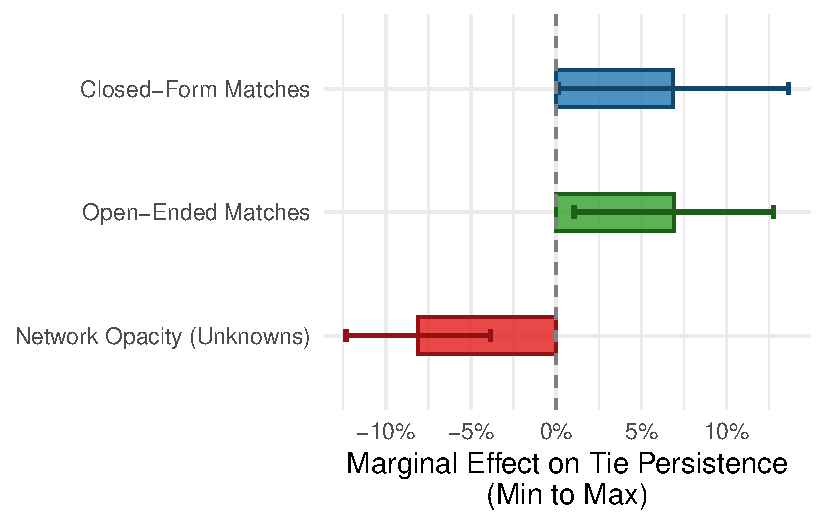
\includegraphics[width=0.8\linewidth,keepaspectratio]{analysis_files/figure-pdf/fig-combined-1.pdf}
\caption{\label{fig-combined}Marginal Effects of Cultural Matching and Network Opacity on Tie Persistence. Note: Estimates represent the average marginal effect on the probability of tie persistence.}
\end{figure}

\newpage
\begin{figure}[htbp]
\centering
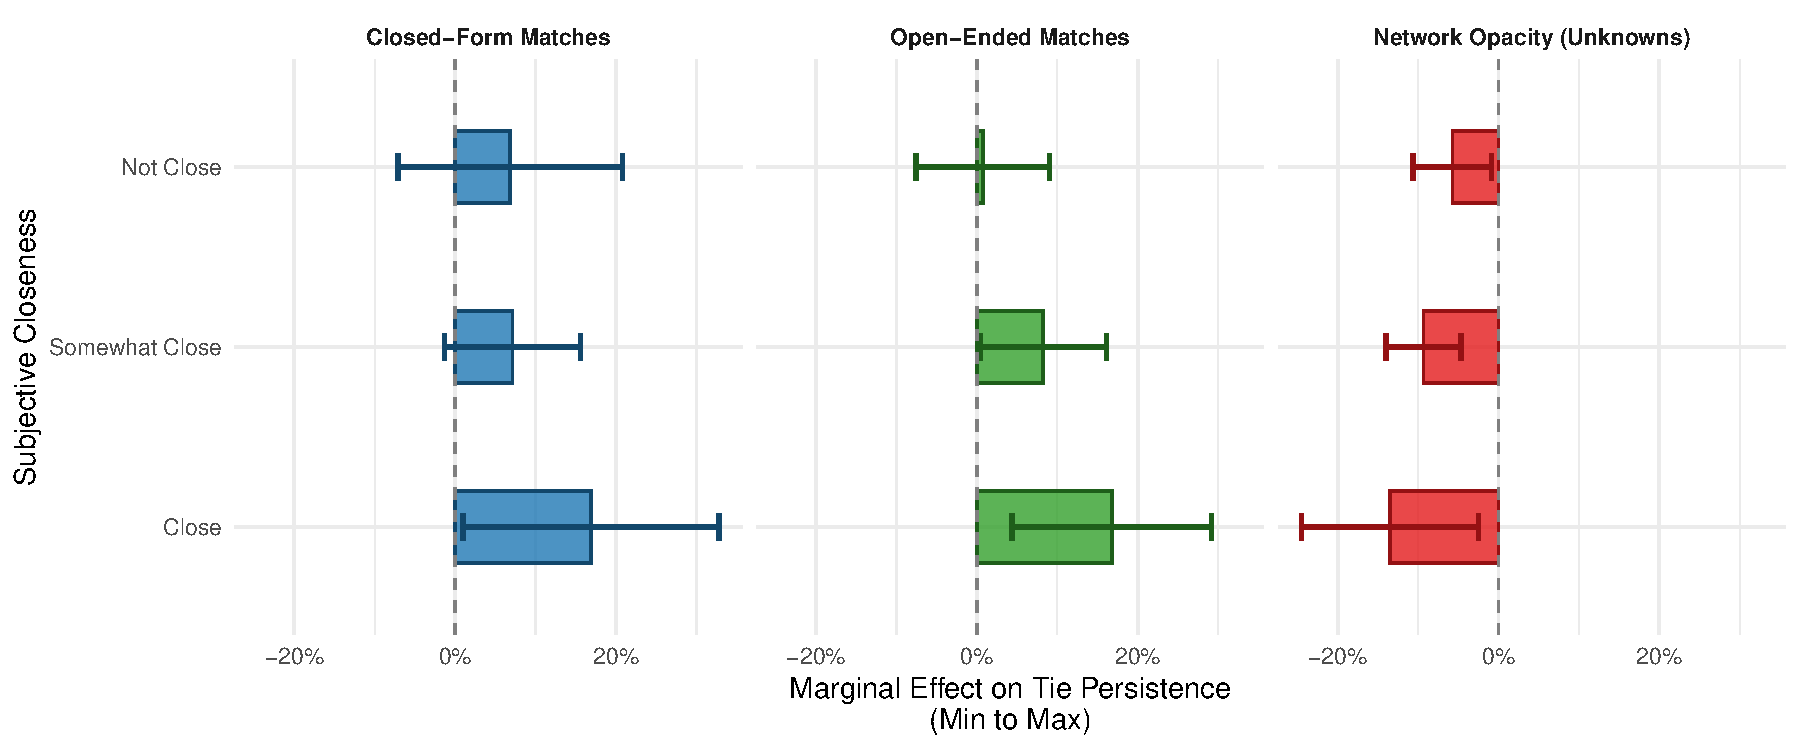
\includegraphics[width=\linewidth,keepaspectratio]{analysis_files/figure-pdf/fig-closeness-interactions-1.pdf}
\caption{\label{fig-closeness-interactions}Marginal Effects of Cultural Matching and Network Opacity on Tie Persistence by Subjective Closeness. Note: Estimates represent the average marginal effect on the probability of tie persistence.}
\end{figure}
\newpage

\section*{Tables}
(Tables inserted dynamically via Quarto/R)

\newpage
\bibliographystyle{plainnat}
\bibliography{manuscript_citations}

\end{document}
